\documentclass[aspectratio=169,11pt]{beamer}

\usetheme{default}
\usefonttheme{professionalfonts}
\setbeamertemplate{navigation symbols}{}
\setbeamertemplate{footline}[frame number]

\definecolor{ink}{HTML}{1F2933}
\definecolor{accent}{HTML}{2A78D6}
\definecolor{rf}{HTML}{2A78D6}
\definecolor{xgb}{HTML}{EB6834}
\definecolor{enet}{HTML}{1BAF7A}
\definecolor{muted}{HTML}{6B7280}
\definecolor{warn}{HTML}{B45309}
\setbeamercolor{normal text}{fg=ink}
\setbeamercolor{frametitle}{fg=accent}
\setbeamercolor{title}{fg=accent}
\setbeamercolor{structure}{fg=accent}
\setbeamerfont{frametitle}{series=\bfseries}

\usepackage{booktabs}
\usepackage{array}
\usepackage{graphicx}
\usepackage{pgfplots}
\pgfplotsset{compat=1.18,
  % Shared look for the bar charts: sans-serif ticks, one swatch per legend entry.
  deckbars/.style={
    tick label style={font=\sffamily\small},
    yticklabel={$\mathsf{\pgfmathprintnumber{\tick}}$},
    label style={font=\sffamily},
    legend image code/.code={\draw[##1] (0cm,-0.1cm) rectangle (0.25cm,0.12cm);}}}
\usetikzlibrary{positioning}

% Figures live in results/figures/ and are produced by the notebooks.
\graphicspath{{../results/figures/}}

\newcommand{\takeaway}[1]{\par\vspace{0.6em}{\color{accent}\textbf{Takeaway:}} #1}
\newcommand{\caveat}[1]{\par\vspace{0.4em}{\color{warn}\textbf{Caveat:}} #1}

\title{Remaining Useful Life of Turbofan Engines}
\subtitle{Phase 1: engineered features and classical ML on NASA C-MAPSS FD001}
\author{cmapss-rul-hybrid team}
\date{Phase 1 review}

\begin{document}

\begin{frame}
  \titlepage
\end{frame}

% ---------------------------------------------------------------- Problem
\begin{frame}{The problem}
  \begin{itemize}
    \item Predict \textbf{remaining useful life (RUL)}: how many operating
      cycles an engine has left before failure, from its sensor history.
    \item Maintenance is scheduled on this number: predicting too much life
      risks a failure in service, too little wastes engine life.
    \item Project question: do \textbf{hand-engineered degradation features}
      with classical regressors (Phase 1) or \textbf{sequence models} that
      learn from raw sensor windows (Phase 2) predict RUL better?
  \end{itemize}
  \vspace{0.5em}
  \begin{block}{Phase 1 deliverable}
    A leakage-free baseline on FD001: Random Forest, XGBoost and Elastic Net,
    each trained on raw inputs and on engineered features, scored on the
    official test engines.
  \end{block}
\end{frame}

% ---------------------------------------------------------------- Data
\begin{frame}{Data: NASA C-MAPSS}
  \begin{columns}[T]
    \begin{column}{0.52\textwidth}
      \small
      \begin{tabular}{lcccc}
        \toprule
        Subset & Cond. & Faults & Train & Test \\
        \midrule
        \textbf{FD001} & 1 & 1 & 100 & 100 \\
        FD002 & 6 & 1 & 260 & 259 \\
        FD003 & 1 & 2 & 100 & 100 \\
        FD004 & 6 & 2 & 249 & 248 \\
        \bottomrule
      \end{tabular}
      \vspace{0.6em}

      {\footnotesize Engines per split. Simulated data, Saxena et al.\ (2008).}
    \end{column}
    \begin{column}{0.46\textwidth}
      \small
      \begin{itemize}
        \item One row per engine cycle: \texttt{unit}, \texttt{cycle},
          3 operating settings, 21 sensors.
        \item Training engines run to failure; test engines stop early.
        \item Training target: final cycle $-$ current cycle.
        \item Test: scored once per engine, at its \textbf{last cycle},
          against \texttt{RUL\_FD001.txt}.
      \end{itemize}
    \end{column}
  \end{columns}
  \takeaway{FD001 (one operating condition, one fault) is the Phase 1 subset;
  20,631 training rows and 13,096 test rows.}
\end{frame}

% ---------------------------------------------------------------- EDA
\begin{frame}{EDA 1: lifetimes vary widely, so split by engine}
  \begin{columns}[c]
    \begin{column}{0.55\textwidth}
      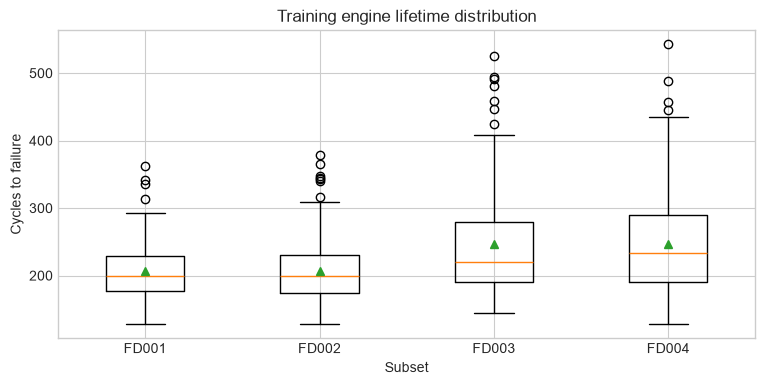
\includegraphics[width=\linewidth]{eda_lifetimes.png}
    \end{column}
    \begin{column}{0.43\textwidth}
      \small
      \begin{itemize}
        \item FD001 lifetimes: 128 to 362 cycles, median 199.
        \item Rows of one engine are strongly related, so a row-level split
          would leak an engine into both train and validation.
        \item The long right tail makes the uncapped target span a wide
          range, which inflates early-life errors.
      \end{itemize}
    \end{column}
  \end{columns}
  \takeaway{All splits are by engine (\texttt{GroupKFold} on \texttt{unit}).}
\end{frame}

\begin{frame}{EDA 2: operating conditions dominate raw sensor levels}
  \centering
  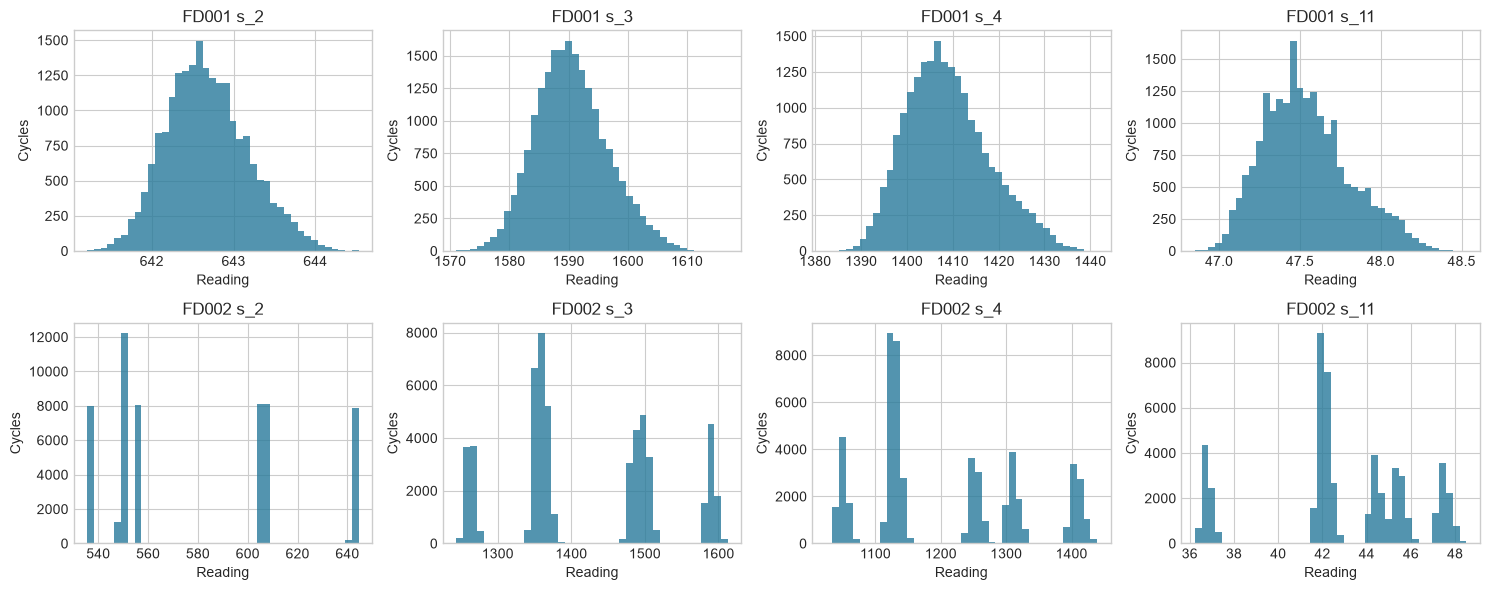
\includegraphics[width=0.72\linewidth]{eda_sensor_hist.png}
  \par\small
  FD001 sensors are unimodal; in FD002 the same sensors split into one mode per
  operating condition, a shift much larger than degradation.
  Six FD001 sensors ($s_1,s_5,s_{10},s_{16},s_{18},s_{19}$) are exactly constant.
  \takeaway{Normalize each sensor within its operating regime, and drop
  constant sensors, fitted on training folds only.}
\end{frame}

\begin{frame}{EDA 3: degradation is slow, then accelerates}
  \centering
  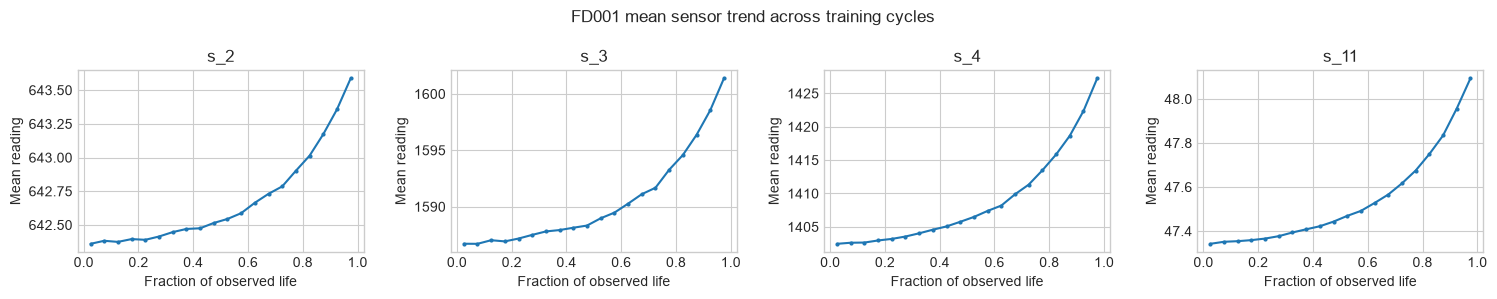
\includegraphics[width=\linewidth]{eda_fd001_sensor_trends.png}
  \par\small\raggedright
  Mean FD001 reading against fraction of observed life. Sensors barely move for
  the first half of life, then rise increasingly steeply.
  \begin{itemize}
    \item Level \emph{and} recent slope carry information
      $\Rightarrow$ rolling mean and rolling slope features.
    \item Early cycles look alike while their true RUL differs widely
      $\Rightarrow$ early-life errors will be large under an uncapped target.
  \end{itemize}
\end{frame}

% ---------------------------------------------------------------- Protocol
\begin{frame}{Evaluation protocol}
  \small
  \begin{columns}[T]
    \begin{column}{0.5\textwidth}
      \textbf{Guardrails (from CONTRIBUTING)}
      \begin{itemize}
        \item Split by engine only, never by row.
        \item Sensor selection, regime clusters and scaling refitted
          \emph{inside} each training fold.
        \item Rolling windows never cross engine boundaries or look ahead.
        \item Uncapped RUL is the primary target; capping is an ablation.
      \end{itemize}
    \end{column}
    \begin{column}{0.48\textwidth}
      \textbf{Tuning and test}
      \begin{itemize}
        \item Grid search, 3 engine-grouped folds over 100 training engines,
          seed 42, selected by CV RMSE.
        \item Best candidate refitted on all 100 training engines.
        \item 100 test engines scored once at their last cycle.
        \item Metrics: RMSE, MAE, NASA score, and RMSE by true-RUL stage:
          late $\le 50 <$ mid $\le 100 <$ early.
      \end{itemize}
    \end{column}
  \end{columns}
\end{frame}

% ---------------------------------------------------------------- Features
\begin{frame}{Feature engineering: 155 predictors per cycle}
  \small
  \begin{columns}[T]
    \begin{column}{0.56\textwidth}
      \begin{enumerate}
        \item \textbf{Selected sensors:} drop exactly constant channels
          $\Rightarrow$ 15 of 21 kept.
        \item \textbf{Regime z-score:}
          $z_{u,t,s}=(x_{u,t,s}-\mu_{r,s})/\sigma_{r,s}$, with K-means regimes
          on the operating settings.
        \item \textbf{Rolling features} over trailing windows
          $w\in\{5,10,20\}$:
          \begin{itemize}
            \item mean $m$ (local level)
            \item least-squares slope $b$ (rate of change)
            \item health change $m-z_{t_0}$ (vs.\ engine's first cycle)
          \end{itemize}
        \item \textbf{Context:} \texttt{cycle}, 3 settings, regime.
      \end{enumerate}
    \end{column}
    \begin{column}{0.42\textwidth}
      \begin{block}{Predictor count}
        $5 + S(1+3W) = 5 + 15\cdot(1+3\cdot3) = 155$
      \end{block}
      \vspace{0.4em}
      \textbf{Raw reference:} \texttt{cycle}, 3 settings and all 21 sensors.
      \vspace{0.4em}

      All features are \textbf{causal}: they use only the current and past
      cycles of the same engine.
    \end{column}
  \end{columns}
\end{frame}

% ---------------------------------------------------------------- Models
\begin{frame}{Models}
  \small
  \begin{tabular}{>{\raggedright\arraybackslash}p{0.17\textwidth}>{\raggedright\arraybackslash}p{0.38\textwidth}>{\raggedright\arraybackslash}p{0.34\textwidth}}
    \toprule
    Model & Why it is here & Grid searched \\
    \midrule
    {\color{rf}\textbf{Random Forest}} &
      Averages deep trees to cut variance; non-linear, no scaling needed,
      predictions stay in the training RUL range. &
      trees $\{50,100\}$, min leaf $\{1,3\}$, \texttt{max\_features}=0.5 \\ \addlinespace[0.6em]
    {\color{xgb}\textbf{XGBoost}} &
      Boosts shallow trees to cut bias; usually the strongest tabular model. &
      trees $\{100,200\}$, depth $\{3,5\}$, learning rate fixed at 0.3 \\ \addlinespace[0.6em]
    {\color{enet}\textbf{Elastic Net}} &
      Linear reference with $\ell_1+\ell_2$ penalty; handles the many
      correlated rolling features; interpretable. &
      $\alpha\{0.1,1.0\}$, $\ell_1$ ratio $\{0.2,0.8\}$, standardized inputs \\
    \bottomrule
  \end{tabular}
  \vspace{0.6em}

  All three minimize squared error, so they estimate the conditional mean RUL.
  The asymmetric NASA score is reported but not optimized.
\end{frame}

% ---------------------------------------------------------------- CV
\begin{frame}{Cross-validation does not separate the models}
  \begin{columns}[c]
    \begin{column}{0.58\textwidth}
      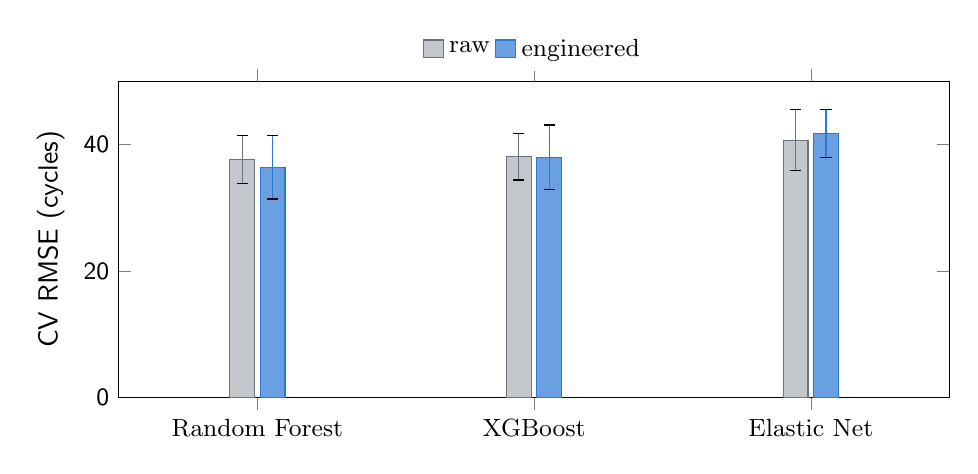
\begin{tikzpicture}
        \begin{axis}[
            width=\linewidth, height=5.6cm,
            ybar, bar width=9pt, deckbars,
            ymin=0, ymax=50,
            ylabel={CV RMSE (cycles)},
            symbolic x coords={Random Forest,XGBoost,Elastic Net},
            xtick=data, enlarge x limits=0.25,
            legend style={at={(0.5,1.03)},anchor=south,legend columns=2,draw=none,font=\small},
            tick label style={font=\small},
            error bars/y dir=both, error bars/y explicit,
          ]
          \addplot[fill=muted!40, draw=muted] coordinates {
            (Random Forest,37.6) +- (0,3.8)
            (XGBoost,38.1) +- (0,3.7)
            (Elastic Net,40.7) +- (0,4.8)};
          \addplot[fill=accent!70, draw=accent] coordinates {
            (Random Forest,36.4) +- (0,5.0)
            (XGBoost,38.0) +- (0,5.1)
            (Elastic Net,41.8) +- (0,3.8)};
          \legend{raw, engineered}
        \end{axis}
      \end{tikzpicture}
    \end{column}
    \begin{column}{0.40\textwidth}
      \small
      Mean $\pm$ standard deviation over 3 engine-grouped folds.
      \begin{itemize}
        \item Every gap between models or feature sets (at most 5.4 cycles)
          is about the size of one fold's standard deviation (3.7 to 5.1).
        \item With only 3 folds, the ranking could change with a different
          seed.
        \item Several selected settings sit on the edge of their grid.
      \end{itemize}
    \end{column}
  \end{columns}
  \takeaway{CV alone does not establish a preferred model or feature set.}
\end{frame}

% ---------------------------------------------------------------- Test
\begin{frame}{Official FD001 test results (uncapped RUL)}
  \centering\small
  \begin{tabular}{l rrr @{\hspace{1.6em}} rrr}
    \toprule
    & \multicolumn{3}{c}{Engineered features} & \multicolumn{3}{c}{Raw inputs} \\
    \cmidrule(r{1.4em}){2-4}\cmidrule{5-7}
    Model & RMSE & MAE & NASA & RMSE & MAE & NASA \\
    \midrule
    Random Forest & 27.55 & \textbf{17.67} & 145{,}410 & \textbf{26.15} & 19.22 & 8{,}414 \\
    XGBoost       & 30.50 & 19.82 & 61{,}202  & 26.84 & 19.19 & 7{,}002 \\
    Elastic Net   & 28.39 & 23.57 & 7{,}777   & 31.08 & 25.80 & \textbf{6{,}903} \\
    \bottomrule
  \end{tabular}
  \par\vspace{0.4em}{\footnotesize 100 test engines, each scored at its last
  recorded cycle. Lower is better. Bold = best in column group.}
  \raggedright\small
  \begin{itemize}
    \item \textbf{No single winner:} raw Random Forest has the lowest RMSE,
      engineered Random Forest the lowest MAE, raw Elastic Net the lowest NASA
      score.
    \item Engineered features lower RMSE only for Elastic Net
      (31.08 $\to$ 28.39); for both tree models they raise it.
  \end{itemize}
  \caveat{One test set of 100 engines and no confidence intervals: a
  difference of 1 to 2 RMSE may not be real.}
\end{frame}

% ---------------------------------------------------------------- Stage
\begin{frame}{Where the errors are: by true-RUL stage}
  \begin{columns}[c]
    \begin{column}{0.58\textwidth}
      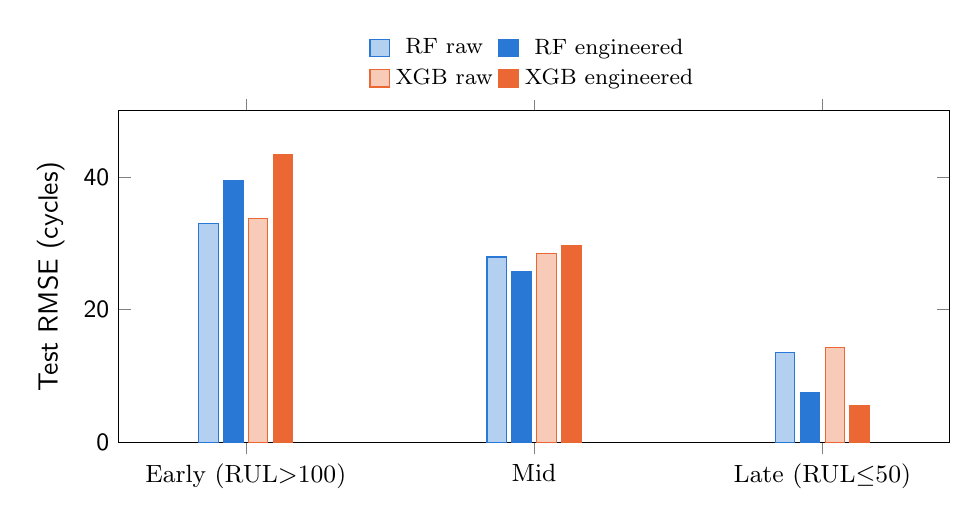
\begin{tikzpicture}
        \begin{axis}[
            width=\linewidth, height=5.8cm,
            ybar, bar width=7pt, deckbars,
            ymin=0, ymax=50,
            ylabel={Test RMSE (cycles)},
            symbolic x coords={Early,Mid,Late},
            xticklabels={{Early (RUL$>$100)},{Mid},{Late (RUL$\le$50)}},
            xtick=data, enlarge x limits=0.22,
            legend style={at={(0.5,1.03)},anchor=south,legend columns=2,draw=none,font=\footnotesize},
            tick label style={font=\small},
          ]
          \addplot[fill=rf!35, draw=rf] coordinates {(Early,32.95) (Mid,27.94) (Late,13.50)};
          \addplot[fill=rf, draw=rf] coordinates {(Early,39.49) (Mid,25.76) (Late,7.52)};
          \addplot[fill=xgb!35, draw=xgb] coordinates {(Early,33.77) (Mid,28.50) (Late,14.32)};
          \addplot[fill=xgb, draw=xgb] coordinates {(Early,43.39) (Mid,29.62) (Late,5.62)};
          \legend{RF raw, RF engineered, XGB raw, XGB engineered}
        \end{axis}
      \end{tikzpicture}
    \end{column}
    \begin{column}{0.40\textwidth}
      \small
      33 early, 34 mid and 33 late engines.
      \begin{itemize}
        \item \textbf{Near failure, engineered features win clearly:}
          RF 13.5 $\to$ 7.5, XGB 14.3 $\to$ 5.6. This is where maintenance
          is scheduled.
        \item \textbf{On young engines they lose:} RF 33.0 $\to$ 39.5,
          XGB 33.8 $\to$ 43.4.
        \item Elastic Net stays poor late (24.8): a linear model cannot follow
          the sharp end-of-life drop.
      \end{itemize}
    \end{column}
  \end{columns}
\end{frame}

% ---------------------------------------------------------------- Pred vs true
\begin{frame}{Predicted vs.\ true RUL (engineered models)}
  \centering
  \vspace{-0.4em}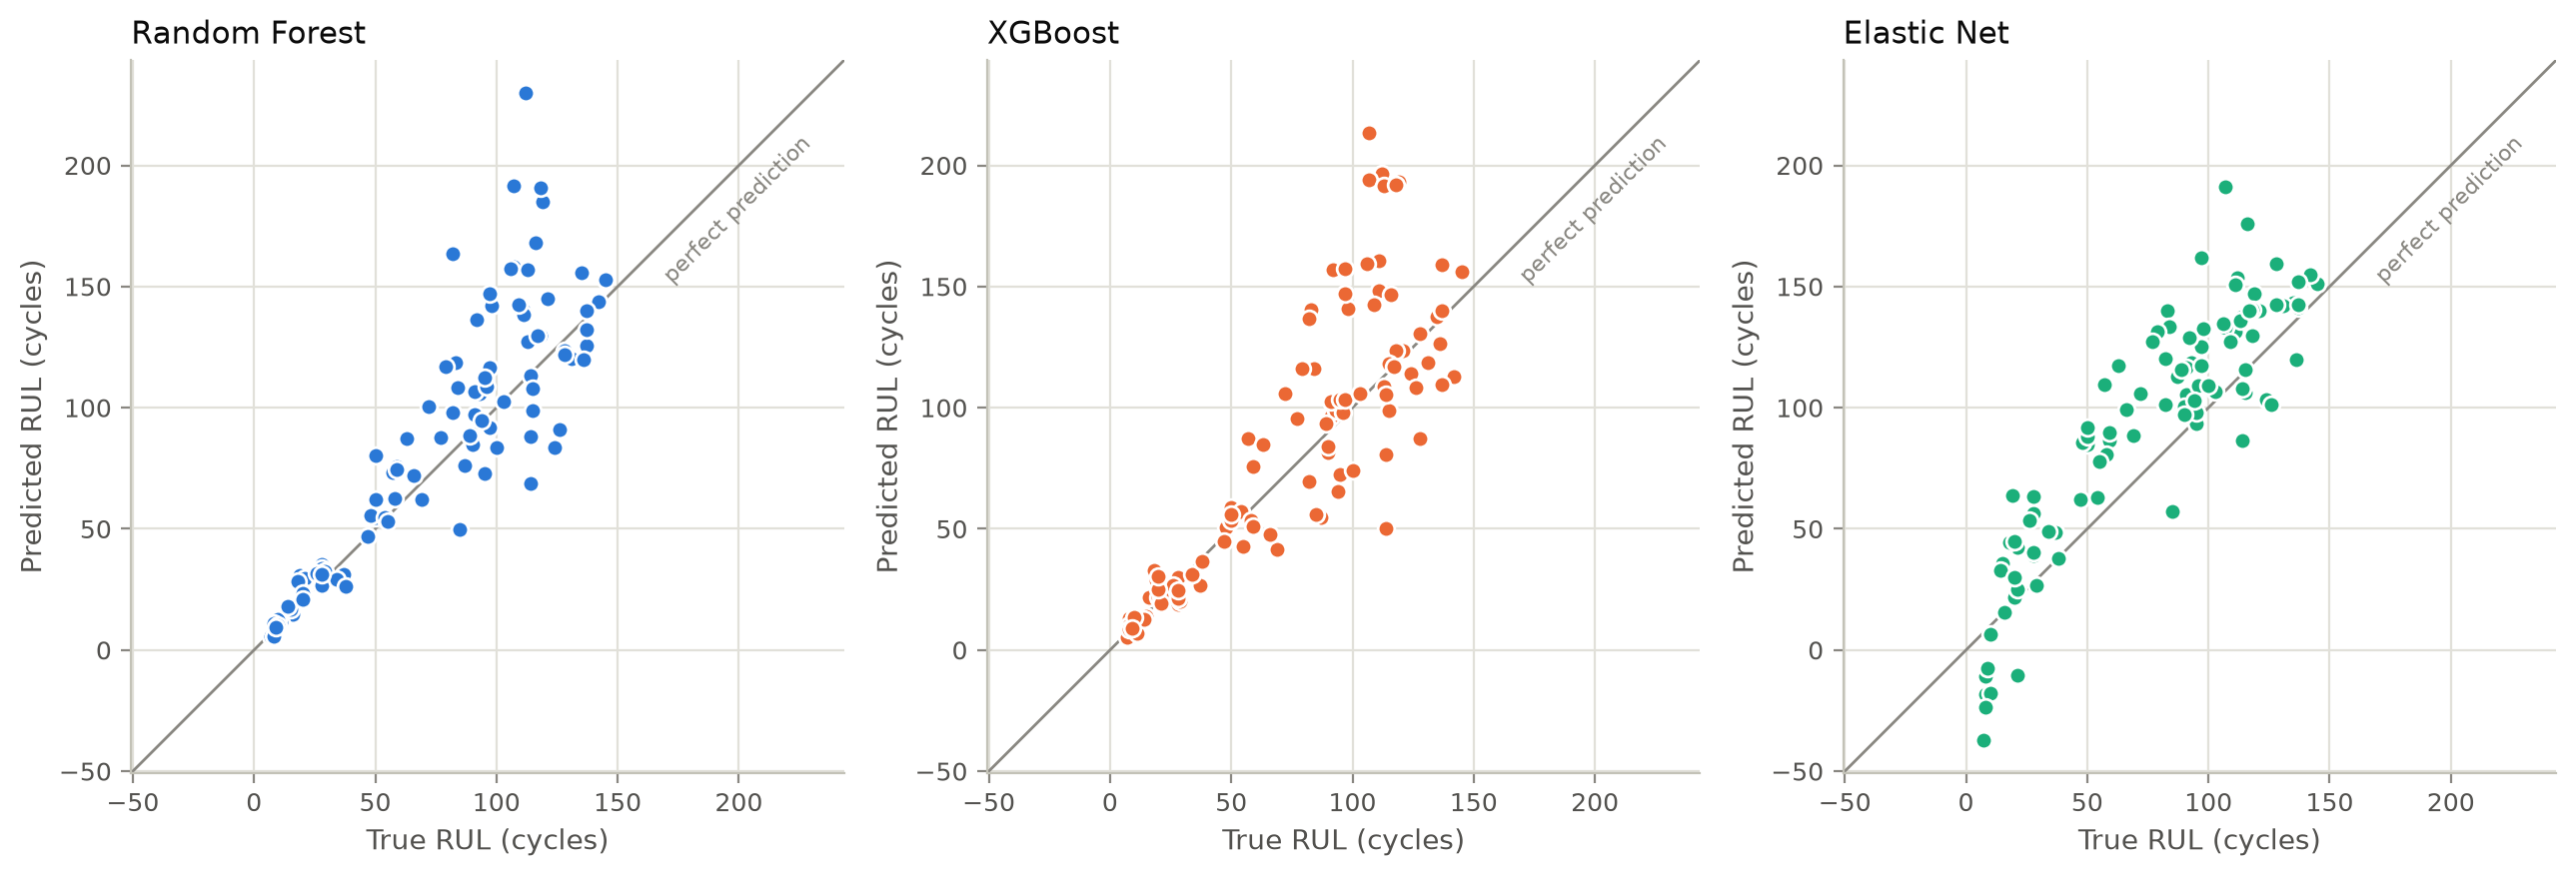
\includegraphics[width=0.92\linewidth]{fd001_test_pred_vs_true.png}
  \par\small\raggedright
  \begin{itemize}
    \item Tight near zero RUL, wide scatter above about 80 cycles.
    \item \textbf{NASA score is driven by single engines:} test engine 1 (31
      cycles seen, 112 left) is predicted at 230 by engineered RF, which is
      92\% of its 145{,}410 score. Read NASA together with RMSE and MAE.
    \item Elastic Net predicts negative RUL for 7 engines (not clipped).
  \end{itemize}
\end{frame}

% ---------------------------------------------------------------- Capping
\begin{frame}{The headline depends on the target definition}
  \small
  \textbf{Why young engines are hard.} With an uncapped target, an engine at
  cycle 31 that still looks new could have 100 or 300 cycles left; the sensors
  cannot tell. The models fall back on age: Tree SHAP attributes far more of
  each engineered prediction to \texttt{cycle} than to any sensor.

  \vspace{0.6em}
  {\color{accent}\textbf{Preliminary check: Random Forest trained with RUL capped at 125}}\par\vspace{0.3em}
    \begin{tabular}{lcc}
      \toprule
      Training target & Engineered & Raw \\
      \midrule
      Uncapped (primary) & 27.55 & \textbf{26.15} \\
      Capped at 125      & \textbf{16.4} & 18.7 \\
      \bottomrule
    \end{tabular}
    \quad
    \begin{minipage}[c]{0.48\linewidth}
      \raggedright\footnotesize Test RMSE against the true (uncapped) test RUL.
      Random Forest only, one run; not yet in \texttt{results/metrics/}.
    \end{minipage}
  \caveat{Under a capped target the raw-vs-engineered ranking \textbf{flips}.
  So ``engineered features do not help'' is not a safe conclusion. The cap of
  125 must be justified from training data, not chosen on the test set.}
\end{frame}

% ---------------------------------------------------------------- Limits
\begin{frame}{Limitations of Phase 1}
  \small
  \begin{itemize}
    \item \textbf{CV is scored differently from the test:} CV scores every
      training cycle (RUL up to 361), the test only the last cycle (RUL at
      most 145). This is why CV RMSE (36 to 42) exceeds test RMSE (26 to 31),
      and it means tuning optimizes a different objective.
    \item \textbf{Small grids:} two values per hyperparameter, several winners
      on a grid edge, XGBoost learning rate not tuned.
    \item \textbf{No uncertainty:} 3 folds and 100 test engines, with no
      confidence intervals or paired tests.
    \item \textbf{One subset:} only FD001 (one condition, one fault) is
      evaluated; regime normalization has not yet been tested on FD002/FD004.
    \item \textbf{No feature ablations yet:} we do not know which feature
      groups help, or how much \texttt{cycle} alone explains.
  \end{itemize}
\end{frame}

% ---------------------------------------------------------------- Next
\begin{frame}{Next steps}
  \small
  \begin{columns}[T]
    \begin{column}{0.5\textwidth}
      \textbf{Close out Phase 1}
      \begin{enumerate}
        \item Run the capped-target ablation for all six models and commit it.
        \item Score CV on last-cycle-like samples to match the test.
        \item Widen grids; tune the XGBoost learning rate.
        \item Feature ablations: drop \texttt{cycle}, add a long window.
        \item Bootstrap confidence intervals over test engines.
      \end{enumerate}
    \end{column}
    \begin{column}{0.48\textwidth}
      \textbf{Phase 2: sequence models}
      \begin{itemize}
        \item LSTM / temporal CNN / Transformer on fixed-length sensor
          windows built inside engine boundaries.
        \item Same splits, same metrics, same last-cycle scoring.
        \item \textbf{Bar to beat:} 26.15 RMSE overall and about 6 to 8 RMSE
          in the late stage (uncapped).
      \end{itemize}
    \end{column}
  \end{columns}
\end{frame}

\begin{frame}{Summary}
  \begin{itemize}
    \item A leakage-free, engine-grouped baseline exists for FD001, with six
      models scored on the official test engines.
    \item Best uncapped test RMSE: \textbf{26.15} (raw Random Forest); best
      late-stage RMSE: \textbf{5.6} (engineered XGBoost).
    \item Engineered features clearly help near failure and hurt on young
      engines; overall rankings are within noise.
    \item The raw-vs-engineered conclusion depends on how RUL is defined, so
      Phase 1 is not finished until the capped ablation is run properly.
  \end{itemize}
  \vspace{1em}
  \centering{\Large Questions?}
\end{frame}

% ---------------------------------------------------------------- Backup
\appendix
\begin{frame}{Backup: prediction trajectories}
  \centering
  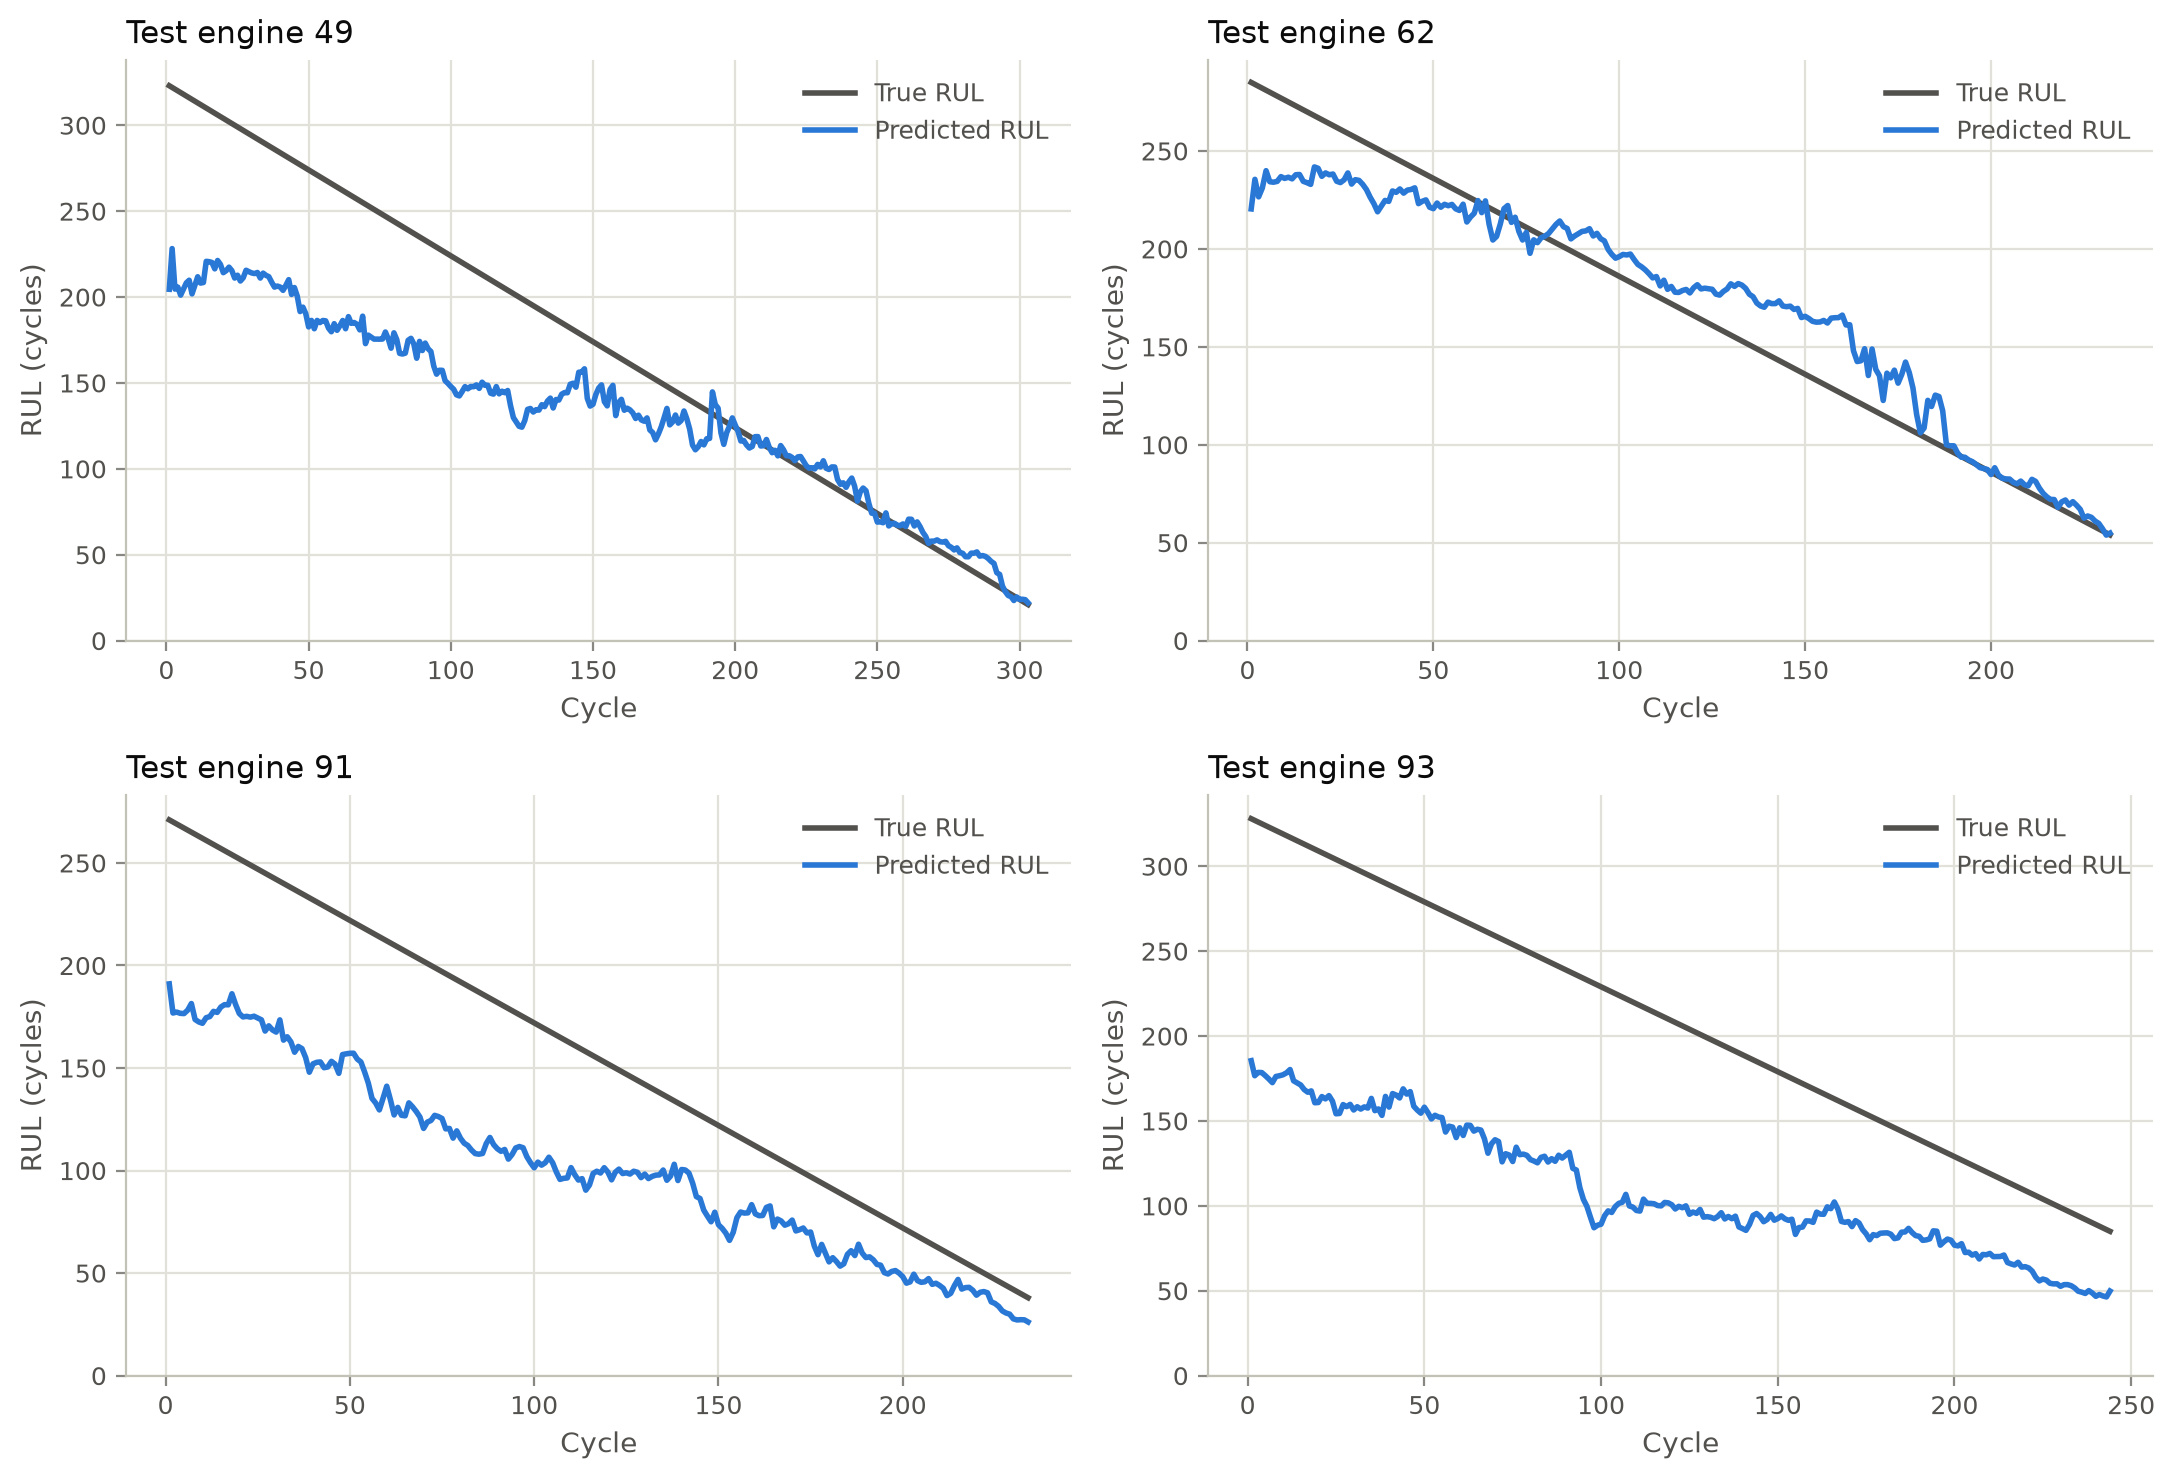
\includegraphics[height=0.78\textheight]{fd001_test_trajectories.png}
  \par\footnotesize The four test engines with the longest recorded histories,
  engineered model with the lowest test RMSE.
\end{frame}

\begin{frame}{Backup: operating settings in FD002 and FD004}
  \centering
  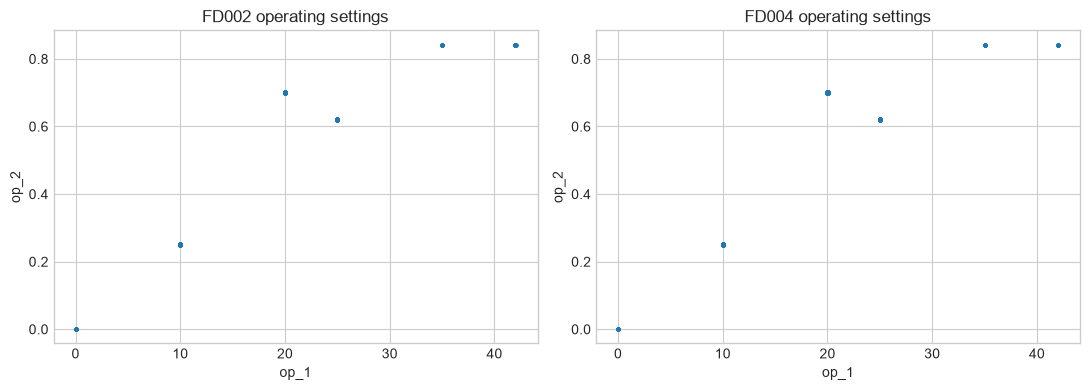
\includegraphics[width=0.85\linewidth]{eda_op_settings.png}
  \par\small Six tight clusters, one per simulated flight condition. This is
  what the K-means regime step recovers.
\end{frame}

\end{document}
